% *******************************************************************************
% * Copyright (c) 2007 by Elexis
% * All rights reserved. This document and the accompanying materials
% * are made available under the terms of the Eclipse Public License v1.0
% * which accompanies this distribution, and is available at
% * http://www.eclipse.org/legal/epl-v10.html
% *
% * Contributors:
% *    G. Weirich - initial implementation
% *
% *  $Id: mitmachen.tex 2651 2007-06-28 19:46:29Z rgw_ch $
% *******************************************************************************
% !Mode:: "TeX:UTF-8" (encoding info for WinEdt)
%
% Dieses Dokument behandelt die Möglichkeiten, an Elexis mitzuwirken

\chapter{Bases}
\section{Introduction}
Dans cette partie du Manuel nous parlons des différentes possibilités de contribuer au développement de Elexis. Puisque il faut pour le développement de Elexis certains instruments il y aura quelques parties assez techniques. Ne vous laissez pourtant pas décourager car premièrement les choses se voient souvent plus compliquées qu'elle ne le sont et en plus nous sommes volontiers prêts à vous aider de prendre pied dans l'affaire.
\section{Eclipse}
\label{Eclipse}
Eclipse (\href{http://www.eclipse.org}{www.eclipse.org}) \index{Eclipse} est l'environement de développement idéal pour Elexis puisque Elexis lui-même est une application Eclipse. Eclipse est un instrument puissant qui ne peut être utlisé pas seulement pour a programmation mais entre autres aussi pour écrire une documentation. On peut télécharger gratuitement Eclipse pour Windows, Linux, Mac ou d'autres systèmes d'exploitation.Vous nécessitez la variante  \glqq Eclipse SDK\grqq{} pour votre système d'exploitation. L'installation est facile : Il suffit de décompresser le fichier d'archivation quelque part.
\section{Système de contrôle de version}
Les sources, donc les racines du projet entier de \textit{elexis}  se trouvent dans un système de contrôle de version 
\index{système de contrôle de version} réspectivement dans un 
\glqq revision control system\grqq. \index{RCS}. Un système de contrôle de version est un système de dépôt qui est capable de sauvegarder des fichiers de tout genre  dans une mémoire spécifique qui s'appelle \glqq
Repository\grqq \index{Repository}. Deux choses marquent la particularité de ce système :
\begin{itemize}
\item Toutes les versions de toutes les fichiers sont sauvegardées et marquées avec la date et l'identificateur de celui qui l'a crée ou modifié. On peut revenir à tout moment à une version quelconque d'un fichier . Chaque modification d'un fichier provoque la cération d'un nouveau fichier.
\item Si plusieures personnes font simultanément des modifications d'un fichier, ces modifications seront si possible réunies automatiquement. Ceci n'est pas possible lorsque plusieures personnes travaillent par hasard juste au même endroit d'un fichier. Dans ce cas de figure le système de contrôle de version marquera l'endroit comme conflit et celui doit être résolu ensuite manuellement.
\end{itemize}

Le système de contrôle de version que nous utilisons pour Elexis est les système  \glqq
Sub\-ver\-sion\grqq (\href{http://subversion.tigris.org}{subversion.tigris.org}) qui est assez nouveau. \index{Subversion}
Le 'Repository' se trouve sur un serveur du 'host' OpenSource \href{http://www.sourceforge.net}{Sourceforge} (\glqq forge de sources\grqq).

Puisque Elexis est un système OpenSource tout accès de lecture sur le 'Repository' est complètement libre. Il est donc facilement possible de télécharger les sources sur votre ordinateur et d'y produire votre propre version d'Elexis.   

Pour protéger le projet contre du vandalisme on ne peut par contre pas donner un \textit{accès d'écriture} sans contrôle. Même si tout le monde peut faire des changements au niveau du texte il n'est pas possible pour tout le monde de les télécharger vers le 'Repository'. Toutefois, nous donnons aux personnes qui montrent sérieusement intérèt au développement de Elexis un accès d'écriture.

\section{Moyens nécessaires}
Pour pouvoir accéder aux fichiers dans le 'Repository' vous nécessitez un \textit{Subversion Client}. Ceci peut être selon votre environement un client intégré par exemple pour Eclipse ou un client avec ligne de commandement. Nous décrivons ici l'installation du 'Subversion Client' intégré pour Eclipse qui peut être téléchargé comme \textit{Plugin} pour Eclipse.
\subsection{Installation du client Subclipse dans Eclipse}
\label{subclipse}\index{Subversion!Plugin pour Eclipse}
\begin{itemize}
  \item Séléctionnez dans Eclipse le menu \textsc{Help -- Software~Updates -- Find
  and install}
  \item Sélectionnez ensuite le point \textit{Search for new features to install} et cliquez sur \textsc{Next}
  \item Choisissez \textsc{New Remote Site}
  \item Introduisez comme \glq Name\grq : Sub\-clipse et pour \glq URL\grq:
  http://subclipse.tigris.org/update\_1.2.x
  \item Séléctionnez sous \glqq Select features to install\grqq Subclipse et cliquez sur \textsc{Next}. Après avoir accepté les conditions de licence vous pouvez installer Subclipse.

\end{itemize}
\subsection{client avec ligne de commandement pour subversion}
\label{subversionclient}\index{Subversion!client avec ligne de commandement}
Vous pouvez naturellement aussi accéder au 'Subversion-Repository' sans devoir installer d'abord Eclipse. Peut-être vous préférez travailler avec un autre environement de développement ou vous voulez que télécharger les sources de documentation pour les travailler avec un autre \Instrument-TeX. Dans les deux cas vous nécessitez un client avec ligne de commandement pour subversion. Vous pouvez le télécharger pour votre système d'exploitation chez \href{http://subversion.tigris.org}{subversion.tigris.org}.

\section{permier téléchargement des sources}
\subsection{avec Eclipse}
Ouvrez dans Eclipse la perspective-Subversion (\textsc{Window -- Open
Perspective -- Other -- SVN Repository Exploring}). Avec la touche droite vous cliquez ensuite dans la fenêtre \glqq SVN Repository\grqq{} et séléctionnez \textsc{New --
Repository Location}. Veuillez introduire le URL suivant:
\begin{quote}https://elexis.svn.sourceforge.net/svnroot/elexis/trunk\end{quote}. Si tout marche comme prévu le symbole du 'Repository' devait apparaître avec ce nom dans la fenêtre. Veuillez cliquer sur le signe Plus à gauche pour voir tous les sous-projets de Elexis. Séléctionnez un ou plusieurs projets qui vous intéressent, cliquez avec la touche droite et choisissez \textsc{checkout}. Ce processus dure quelque temps (quelques minutes jusqu'à un quart d'heure pendant laquelle \glqq rien\grqq{} ne semble se passer. Gardez toujours le préréglage lors des demandes de précisions et cliquez \textsc{Next} réspectivement \textsc{finish}.
\subsection{sous un client avec ligne de commandement}
Ouvrez dans le classeur où vous pensez installer le projet Elexis une ligne de commande et introduisez le suivant : \begin{quote}svn checkout https://elexis.svn.sourceforge.net/svnroot/elexis/trunk\end{quote}. Ceci ferait un téléchargement de tout le projet. Si vous ne voulez télécharger qu'un seul sous-projet comme par exemple la documentation vous pouvez introduire : \begin{quote}svn checkout https://elexis.svn.sourceforge.net/svnroot/elexis/trunk/dokumentation\end{quote}. Pour toutes les autres possibilités veuillez consulter l'excelente documentation pour Subversion qui est à votre disposition.

\section{travailler avec des sources}
Le \glqq checkout\grqq{} qu'on vient de décrir n'est nécessaire que lors du premier téléchargement du projet. Plus tard vous startez chaque cycle de travail avec un \glqq update\grqq, travaillez les sources et procédez à la fin à un \glqq commit\grqq{} (si vous avez les droits nécessaires.\footnote{Pour recevoir les droits du 'Commit' vous devez demander quelqu'un de l'administration du projet et il vous faut un account chez Sourceforge. } )
\subsection{update}
\begin{itemize}
  \item dans Eclipse: Cliquez droit sur le projet en question et séléctionnez \textsc{Team-Update}.
  \item ligne de commandement: Changez dans le registre du projet et introduisez \textsc{svn update}. Ceci télécharge sur votre ordinateur tous les changements qui ont été faits entre temps peut être par d'autres personnes .
\end{itemize}
\subsection{commit}
\begin{itemize}
  \item dans Eclipse: Cliquez droit sur le projet en question et séléctionnez \textsc{Team-Commit}.
  \item ligne de commandement: Allez dans le registre du projet et introduisez avec \textsc{svn commit
  -m\glqq la description de votre commits\grqq}. Ceci réécrit les changements dans le 'Repository' et les marque avec la description voulu.
\end{itemize}


\chapter{programmer}
\section{Qui peut participer?}
\begin{itemize}
  \item Celui qui maîtrise ou veut apprendre à maîtriser Java et SWT (Standart Widget Toolkit) 
  \item Celui qui veut améliorer ou développer le noyau du système Elexis
  \item Celui qui veut développer des Plugins pour des fonctionnalités spécifiques
\end{itemize}
\section{Comment est-ce qu'on peut participer?}
Nous préconisons absolument Eclipse comme plateforme de développement. Naturellement on peut travailler Elexis aussi par d'autres IDE mais en ce cas beaucoup de choses deviennent plus compliquées.
Veuillez suivre les instructions mentionnées (voir \pageref{Eclipse}))pour installer Eclipse et le Plugin Subclipse.

Puisque le thème \glqq programmation de Elexis\grqq{} dépasserait le cadre de ce manuel nous vous renvoyons vers la page Web du projet Elexis à la section \glqq Developers\grqq{}.

\chapter{Tester}
\section{Qui peut participer? }
Nous sommes intéressés en première ligne à des personnes qui veulent \glqq véritablement\grqq{} utiliser Elexis et qui sont  prêts à investir le temps nécessaire à trouver des éventuelles fautes ou erreurs pour nous les annoncer de la façon la plus pertinente et compréhensible.
\section{De quelle façon on peut participer?}
\label{senderrors}
Au fond il ne vous faut rien d'autre qu'une installation de base. Il est par contre indispensable de remplir correctement la partie \glqq E-Mail\grqq{} sous \textsc{Fichier -- Paramètres}(voir Fig. \ref{fig:mailsettings})
\begin{figure}[htp]
\begin{center}
  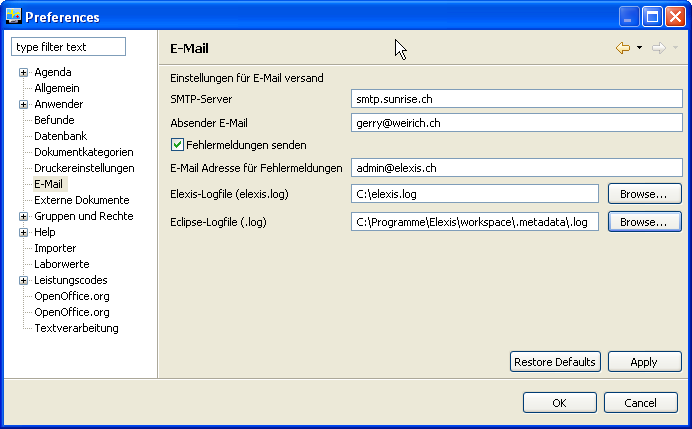
\includegraphics[width=150mm]{images/mailsettings}
  \caption{Einstellungen für Fehlermeldungen}
  \label{fig:mailsettings}
\end{center}
\end{figure}
\section{Procédé lorsqu'on trouve une faute}

Aucun logiciel peut être sans faute. Ceci vaut pour des programmes ClosedSource comme ceux  OpenSource. Dans les produits OpenSource on trouve en général une 'culture d'erreur' qui permet des corrections souvent plus rapides et adéquates.
\subsection{Quelles erreurs doivent êtres annoncées?}
Nous sommes d'avis que la notion \glqq erreur\grqq{} ne doit pas être comprise trop restreinte. Nous considerons un comportement quelconque du logiciel qui ne correspond pas à ce que vous attendez suffisant pour nous l'annoncer.
\subsection{Feed-back simple}
Si vous trouvez une erreur ou un \glqq comportement bizarre\grqq{} du logiciel, essayez tout d'abord à réproduire le phénomène. Séléctionnez ensuite le menu \textsc{aide -- envoyer message d'erreur}. Décrivez dans le dialogue suivant de la façon la plus détaillée les pas qui permettent à reproduire l'erreur. En nous envoyant le mail vous nous envoyez automatiquement aussi deux Logfiles qui ne contiennent naturellement pas des données personnelles ou confidentielles (vous pouvez les regarder à tout moment par un éditeur de texte) mais seul des informations sur des interna du logiciel au moment donné. 
\subsection{Publication des erreurs}
Si vous avez l'impression que l'erreur que vous venez de découvrir est d'une grande importance, vous pouvez introduire l'information concernant cette erreur directement dans le Bug-Tracker de Sourceforge.

\section{procédé pour demande de fonctionnalité supplémentaire du programme}

\chapter{Traduction}
Au fond Elexis est un programme polyglotte. La majorité des textes peuvent être échangés avec facilité et sans connaissance de programmation contre l'équivalent traduit dans une autre langue. Par contre il est possible que les difficultés se montreront comme souvent dans les détails. Faute d'expérience nous ne pouvons pas dire si Elexis pourrait fonctionner parfaitement sans problème dans une autre langue que l'Allemand et le Français. 
Le Team autour Elexis n'a jusqu'alors pas fait d'effort pour lancer la traduction de Elexis car d'autres travaux ont une priorité supérieure. Nous sommes par contre disponible de soutenir selon nos possibilités celui qui veut se lancer dans une traduction. Nous répétons encore une fois qu'il ne faut pas avoir des connaissances de programmation pour faire la traduction de Elexis.

\chapter{Documentation}
\section{Qui peut participer?}
\label{dokumentation}
Réponse très courte: Toute personne qui veut contribuer à la documentation de Elexis est cordialement bienvenu. Nous nécessitons des chapitres de documentation, des modes d'emploies (quick guide), rapports d'expériences et autres.

\section{Comment peut-on participer?}
\subsection{Des articles séparés}
Veuillez envoyer simplement votre article vers dokumentation@elexis.ch
\subsection{un engagement plus important}
Si vous voulez corriger des articles ou introduire plusieurs éléments de documentation, il serait plus facile de travailler directement sur les textes originaux de la documentation. 

\subsubsection{texte original et conditions:}
La documentation de Elexis se base sur des textes originaux -\TeX. En principe un simple éditeur de texte est suffisant pour travailler les textes originaux. Par contre il est naturellement plus confortable de travailler dans un environement \LaTeX - Entwicklungsumgebung. Sous Windows nous préconisons par exemple MiKTeX \href{http://www.miktex.org}{www.miktex.org}. Sous Mac vous préférez peut-être MacTex
(\href{http://www.tug.org/mactex}{www.tug.org/mactex}) et sous Linux
on trouve teTex comme base standard, qui se trouve jointe à pratiquement toutes les distributions(mais qui doit probablement être installée séparément). Un environement très confortable sous Linux avec surface KDE est kile
\href{http://kile.sourceforge.net/}{kile.sourceforge.net}. Il se trouve souvent déjà inclus dans les distributions et peut par conséquent facilement être installé avec l'outil d'administration des logiciels qui se trouve dans la distribution. 

\subsection{règles}
Certaines règles sont à observer pour que le travail commun sur le texte original ne provoque pas inutilement des conflits :
\begin{itemize}
  \item Les textes doivent si possible être téléchargés vers l'amont directement pour que tout le monde soit toujours à jour.
  \item Un texte téléchargé vers l'amont ne doit pas être terminé ni parfait de point de vu stylistique mais on devait pouvoir le compiler avec latex et PDFLaTeX. Veuillez respecter cette règle de base qui vaut en analogie aussi pour les programmateurs Java :  Ce qui se trouve dans le 'Repository' ne doit pas être sans faute ni parfait mais on \textbf{doit} pouvoir le compiler pour que les autres ne doivent pas perdre leur temps en cherchant les fautes.
  \item Les textes des autres ne doivent être corrigés que très peu. Des différentes personnes ont un style différent et c'est bien comme ça. Il n'est donc pas convenant de faire des corrections stylistiques. Si vous trouvez une faute stylistique qui vous dérrange, contactez l'auteur et demandez-le si vous pouvez corriger. 
  \item Des fautes de frappe peuvent par contre être corrigées à tout moment.
  \item Des textes peuvent toujours êtres complétés par tout le monde.
\end{itemize}

\chapter{Promouvoir le développement}
Vous aimeriez ajouter une fonction spécifique ou un plugin dans Elexis?
Vous nécessitez une fonction de statistique ou de contrôle supplémentaire? En principe: Pas de problème.
Elexis est très ouvert de sorte que tout ceci peut être programmé 'après coup'. Vous pouvez :
\begin{itemize}
  \item engager un programmateur en Java qui peut programmer à ses conditions pour vous ces fonctions souhaitées .
  \item nous expliquer exactement ce que vous souhaitez et nous allons vous faire un devis fiable avec indication de la durée maximale nécessaire pour la réalisation de la programmation. En outre nous poserons la condition de pouvoir mettre à disposition l'élément programmé pour vous aussi au reste de la communauté des utilisateurs d'Elexis. \end{itemize}
